\documentclass{article}
\usepackage{amsmath}
\usepackage{graphicx}
\usepackage[most]{tcolorbox}
\usepackage{listings}
\usepackage{xcolor}

\lstdefinelanguage{CSS}{
    keywords={color, background-color, margin, padding, border},
    sensitive=false,
    morecomment=[l]{//},
    morestring=[b]",
}

\lstdefinelanguage{TypeScript}{
    keywords={import, from, class, extends, public, private, string, number, console, log, export, const, let, return, new},
    sensitive=true,
    morecomment=[l]{//},
    morecomment=[s]{/*}{*/},
    morestring=[b]",
    morestring=[b]',
    morestring=[b]`
}

\lstset{
    basicstyle=\ttfamily\footnotesize,
    keywordstyle=\color{blue}\bfseries,
    stringstyle=\color{red},
    commentstyle=\color{green!70!black},
    numbers=left,
    numberstyle=\tiny\color{gray},
    stepnumber=1,
    numbersep=10pt,
    backgroundcolor=\color{gray!10},
    frame=single,
    breaklines=true,
    showstringspaces=false,
    tabsize=2,
    captionpos=b
}
\title{Fundamental Concepts of Angular}
\author{}
\date{}

\begin{document}

\maketitle

\section*{Definition of Angular}

Angular is an open-source framework developed by Google for creating dynamic web applications. It is based on TypeScript and allows applications to be modularly structured through a component-based architecture with services and modules. Angular simplifies data management, API interactions, state management, and navigation in complex web applications.

\begin{tcolorbox}[colframe=black!70, colback=white, title=Figure 1: Angular Logo, fonttitle=\bfseries]
\centering

\includegraphics[width=0.5\textwidth]{images/Angular_full_color_logo.svg.png}
\end{tcolorbox}

\section*{Angular Architecture}

The architecture of Angular is built on clear separation of responsibilities to ensure scalability and maintainability. The main building blocks of this architecture are: \textbf{modules}, \textbf{components}, \textbf{services}, along with other entities like \textbf{directives} and \textbf{pipes}.
\begin{tcolorbox}[colframe=black!70, colback=white, title=Figure 2: Angular Architecture, fonttitle=\bfseries]
\centering
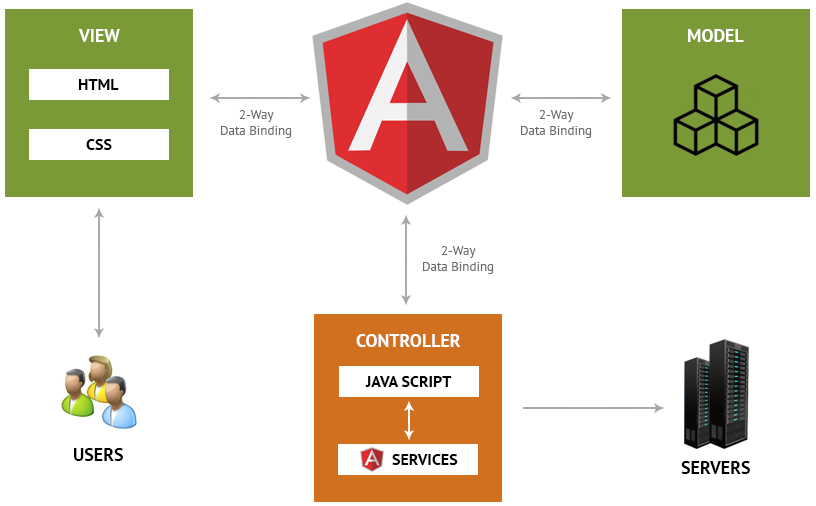
\includegraphics[width=\textwidth]{images/MVC-Architecture-is-Perfect.jpg}
\end{tcolorbox}

The goal of this section is to understand how these elements interact to form a cohesive Angular application.

\section{Overview of Angular Architecture}

Angular follows an enhanced \textbf{Model-View-Controller (MVC)} pattern, where:
\begin{itemize}
    \item \textbf{Components} manage the view and capture user actions.
    \item \textbf{Services} handle data manipulation and business logic.
    \item \textbf{Modules} structure and organize functionalities.
\end{itemize}
\begin{tcolorbox}[colframe=black!70, colback=white, title=Figure 3: Angular Architecture, fonttitle=\bfseries]
\centering
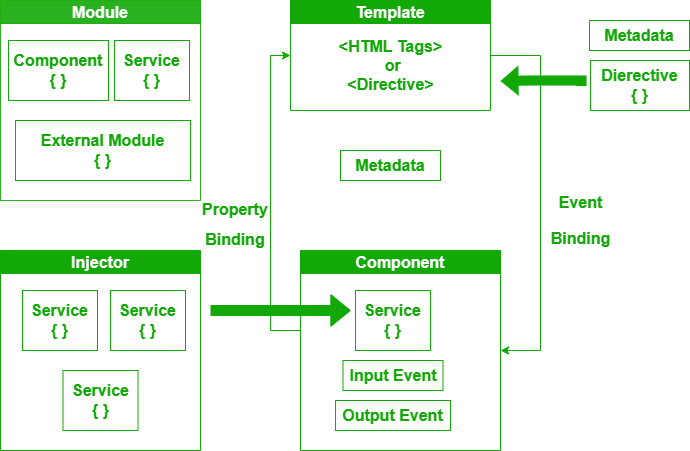
\includegraphics[width=\textwidth]{images/archi.png}
\end{tcolorbox}
This pattern promotes separation of responsibilities for modular development.

\section{Separation of Responsibilities and Data Flow}

\subsection{Modules: The Global Structure}
\begin{itemize}
    \item Modules define the application’s skeleton.
    \item They group components, services, and other entities.
\end{itemize}

\textbf{Relationship with other parts:}  
Modules act as logical containers for grouping related functionalities. For example, an authentication module would contain all components and services related to user management.

\textbf{Tip:} Always start by defining modules before creating associated components and services.

\subsection{Components: The User Interface}
\begin{itemize}
    \item Each component represents a part of the user interface (a button, a form, a page).
    \item A component communicates with services to fetch or process the data to be displayed.
\end{itemize}

\textbf{Data Flow:}  
Data flows \textbf{from the service to the component}, and user actions flow \textbf{from the component to the service}.

\textbf{Tip:} Once the module is configured, begin creating components to design the user interface.

\subsection{Services: Business Logic and Data}
\begin{itemize}
    \item Services are classes dedicated to data management and business processes.
    \item They often use the HTTP module to interact with external APIs.
\end{itemize}

\textbf{Data Flow:}  
Services retrieve or manipulate data and pass it to components.

\textbf{Tip:} After defining the data model (interfaces/classes), develop services to centralize business logic.

\section{Three-Step Data Flow Example}

\begin{enumerate}
    \item \textbf{Defining Modules:}  
    Create a module for a specific functionality (e.g., product management).
    \item \textbf{Creating Services:}  
    Implement a service to fetch product data via an API.
    \item \textbf{Designing Components:}  
    Develop a component that uses the service to display a product list.
\end{enumerate}
\begin{tcolorbox}[colframe=black!70, colback=white, title=Figure 4: Data Flow, fonttitle=\bfseries]
\centering
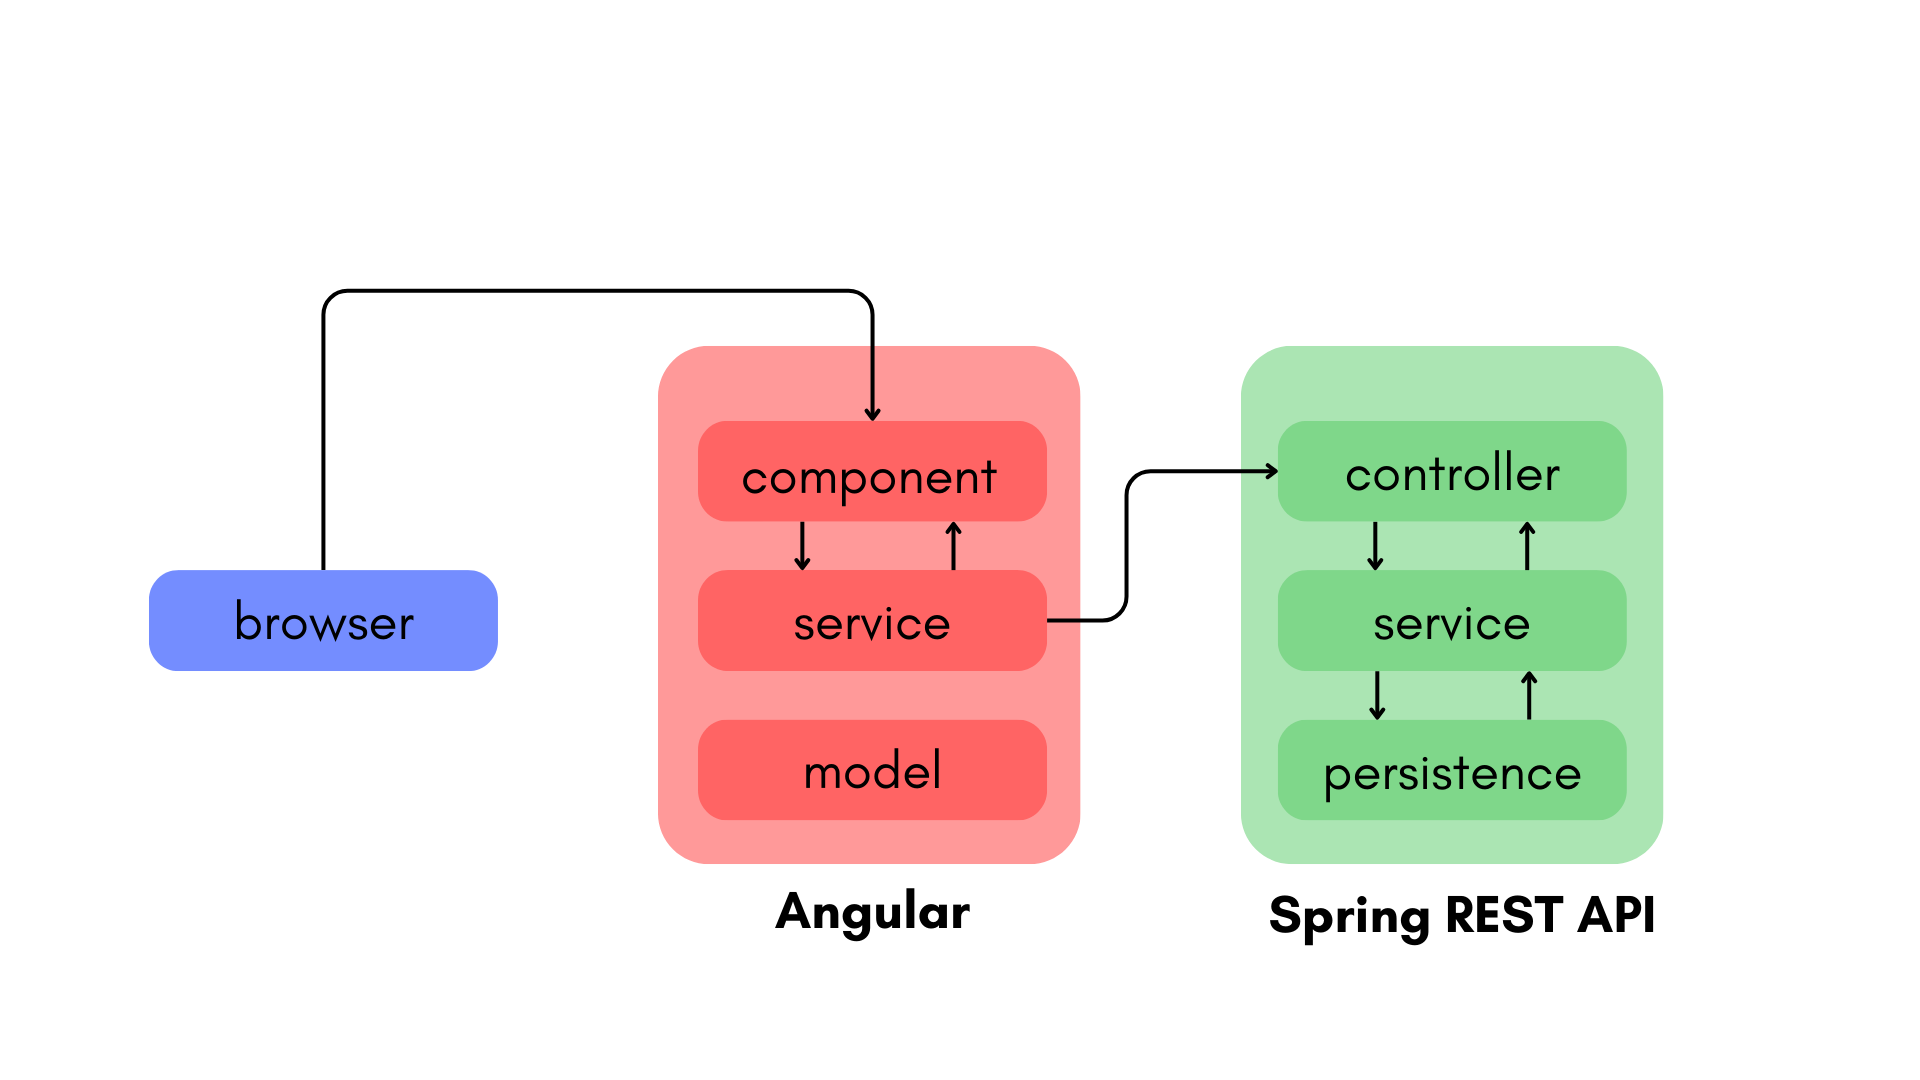
\includegraphics[width=\textwidth]{images/angular_spring_diagram.png}
\end{tcolorbox}

\section{Importance of Data Flow Between Parts}

The order of development is crucial to avoid errors and inefficiencies:
\begin{enumerate}
    \item \textbf{Module:} Structures functionality and facilitates integration.
    \item \textbf{Service:} Manages data and processes related to the functionality.
    \item \textbf{Component:} Displays data to the user and captures user actions.
\end{enumerate}

This flow ensures clean architecture with well-defined responsibilities and maintainable code.
\section*{Modules in Angular: Structure and Functionality}

In Angular, \textbf{modules} play a key role in organizing the application. They allow grouping components, services, directives, pipes, and other modules to make the application modular, reusable, and easily maintainable. Each module is associated with a TypeScript file that serves as the module's entry point, the most important being \textbf{AppModule}, the main module.

\subsection*{1. AppModule: The Application Entry Point}

The \textbf{AppModule} is the base module of any Angular application. It is the module that gets loaded during the application's startup. It groups all the other modules required for the application to function correctly.

\textbf{AppModule Declaration:}  
AppModule is a typical Angular module containing essential information to bootstrap the application, such as component declarations, necessary module imports, services, and dependency injection.

\textbf{Example:}  
\begin{lstlisting}[language=TypeScript, caption={Using a service in a component}, label={lst:typescript-service-usage}]
import { NgModule } from '@angular/core';
import { BrowserModule } from '@angular/platform-browser';
import { AppComponent } from './app.component';

@NgModule({
  declarations: [  // Declare all components used by this module
    AppComponent
  ],
  imports: [  // Import other required modules
    BrowserModule
  ],
  providers: [],  // Declare services
  bootstrap: [AppComponent]  // Component that bootstraps the application
})
export class AppModule { }
\end{lstlisting}

\subsection*{2. Structure of Angular Modules}

An Angular module is defined using the \texttt{@NgModule} decorator, which takes an object with several key properties. These properties configure the module based on the application's specific needs.

\subsubsection*{2.1 Declarations}
The \texttt{declarations} property groups all the \textbf{components}, \textbf{directives}, and \textbf{pipes} used within the module. Every component, directive, or pipe must be declared in a module to be recognized and used.

\begin{itemize}
    \item \textbf{Components:} Represent the user interface.
    \item \textbf{Directives:} Modify the appearance or behavior of a DOM element.
    \item \textbf{Pipes:} Transform the data displayed to the user.
\end{itemize}

\textbf{Example:}  
\begin{verbatim}
@NgModule({
  declarations: [
    AppComponent,
    HeaderComponent,
    FooterComponent
  ]
})
\end{verbatim}

\subsubsection*{2.2 Imports}
The \texttt{imports} property contains a list of \textbf{external modules} that this module uses. This allows grouping functionalities from other modules, such as the routing module or forms module.

\begin{itemize}
    \item For example, you can import modules like \texttt{FormsModule}, \texttt{HttpClientModule}, \texttt{RouterModule}, etc.
\end{itemize}

\textbf{Example:}  
\begin{lstlisting}[language=TypeScript, caption={Using a service in a component}, label={lst:typescript-service-usage}]
import { FormsModule } from '@angular/forms';
import { RouterModule } from '@angular/router';

@NgModule({
  imports: [
    BrowserModule,  // Basic module for the browser
    FormsModule,    // Module for forms
    RouterModule    // Module for routing
  ]
})
\end{lstlisting}

\subsubsection*{2.3 Providers}
The \texttt{providers} property allows declaring the \textbf{services} you want to inject into the application. This enables Angular to inject these services into components and other services via dependency injection.

\begin{itemize}
    \item Services can be provided at the module level or for the entire application using \texttt{providers} in \texttt{@NgModule}.
\end{itemize}

\textbf{Example:}  
\begin{lstlisting}[language=TypeScript, caption={Using a service in a component}, label={lst:typescript-service-usage}]
import { ProductService } from './product.service';

@NgModule({
  providers: [
    ProductService  // Declare the service to be used in the application
  ]
})
\end{lstlisting}

\subsubsection*{2.4 Bootstrap}
The \texttt{bootstrap} property specifies the \textbf{main component(s)} that bootstraps the application. Here, you declare the root component of your application, typically \texttt{AppComponent}.

\begin{itemize}
    \item \texttt{AppComponent} is the component used to initialize the application's user interface.
\end{itemize}

\textbf{Example:}  
\begin{verbatim}
@NgModule({
  bootstrap: [AppComponent]  // Define the component that bootstraps the application
})
\end{verbatim}

\subsection*{3. Complete Example of an Angular Module}

Here is an example of a complete module with the various parts we have discussed:

\begin{lstlisting}[language=TypeScript, caption={Using a service in a component}, label={lst:typescript-service-usage}]
import { NgModule } from '@angular/core';
import { BrowserModule } from '@angular/platform-browser';
import { FormsModule } from '@angular/forms';  // For forms
import { RouterModule } from '@angular/router';  // For routing

import { AppComponent } from './app.component';
import { HeaderComponent } from './header/header.component';
import { FooterComponent } from './footer/footer.component';
import { ProductService } from './services/product.service';

@NgModule({
  declarations: [
    AppComponent,  // Main component
    HeaderComponent,  // Header component
    FooterComponent   // Footer component
  ],
  imports: [
    BrowserModule,  // Basic module for the browser
    FormsModule,    // Module for forms
    RouterModule    // Module for routing
  ],
  providers: [
    ProductService  // Service for managing products
  ],
  bootstrap: [AppComponent]  // Main component that bootstraps the application
})
export class AppModule { }
\end{lstlisting}
\subsection*{4. The Role of \texttt{AppModule} in the Information Flow}

The \textbf{AppModule} acts as the entry point and coordination hub for all the functionalities of the application.  
\begin{itemize}
    \item As soon as the application starts, Angular loads the \textbf{AppModule}.
    \item It \textbf{declares} the components, \textbf{imports} the necessary modules (such as those for forms, HTTP services, etc.), \textbf{provides services} for the application, and \textbf{initializes} the \textbf{main component (AppComponent)}.
\end{itemize}

\subsection*{5. Conclusion}

The architecture of an Angular module allows for efficient and maintainable structuring and organization of functionalities. The structure of a module — \textbf{Declarations}, \textbf{Imports}, \textbf{Providers}, and \textbf{Bootstrap} — is essential for defining how the different parts of the application will interact and be accessible across other modules and components.

\textbf{Practical Tip:} Start by defining your modules to organize the application into independent features. Then, add the necessary components and services, ensuring they are properly injected into the modules.

\section*{Components in Angular: Structure and Functionality}

In Angular, \textbf{components} are the fundamental building blocks for constructing the user interface (UI). Each component represents a \textbf{specific part of the UI}, such as a button, a page, or a form. Components enable the division of the UI into modular, reusable, and easily maintainable elements.

Each Angular component is associated with a \textbf{\@Component decorator}, which provides metadata about the component, including the HTML structure, CSS styles, and TypeScript behavior.

\section*{1. The Role of a Component in Angular}

A \textbf{component} serves to:
\begin{itemize}
  \item \textbf{Manage the user interface} of a specific section of the application (e.g., a form, a navigation bar).
  \item \textbf{Handle user interactions} (e.g., clicks, input in form fields).
  \item \textbf{Communicate with other components or services} to retrieve or manipulate data.
\end{itemize}

In summary, components are the building blocks of an Angular application, and their primary role is to bind the display and business logic.

\section*{2. Using the \@Component Decorator}

The \@Component decorator is a function that configures an Angular component. It is used to define the component's metadata, such as the HTML template, CSS styles, and TypeScript behavior. It also connects a component to a specific module.

The \@Component decorator takes an object with several key properties:
\begin{itemize}
  \item \textbf{selector}: Declares the name of the custom HTML element representing this component in the DOM.
  \item \textbf{templateUrl} or \textbf{template}: A link to the HTML file or inline HTML code used for the component's template.
  \item \textbf{styleUrls} or \textbf{styles}: A link to the CSS file or inline CSS code used for the component's styles.
  \item \textbf{providers}: Declares the services used in this component.
\end{itemize}

\textbf{Example of the \@Component Decorator:}
\begin{lstlisting}[language=TypeScript, caption={Using a service in a component}, label={lst:typescript-service-usage}]

import { Component } from '@angular/core';

@Component({
  selector: 'app-header',  // Declares a custom HTML element
  templateUrl: './header.component.html',  // Link to the HTML template
  styleUrls: ['./header.component.css']   // Link to the CSS file for the component
})
export class HeaderComponent {
  title: string = "Welcome to our website";
}
\end{lstlisting}

\section*{3. Structure of a Component}

An Angular component consists of three main files:
\begin{enumerate}
  \item \textbf{HTML (Template)}: Defines the component's user interface.
  \item \textbf{CSS (Styles)}: Defines the styles associated with the component's interface.
  \item \textbf{TypeScript (Class)}: Contains the component's business logic, manages data, and handles user events.
\end{enumerate}

\subsection*{3.1 The HTML File (Template)}

The HTML file defines the structure of the user interface. It can include basic HTML tags as well as Angular directives for data binding and event handling.

\textbf{Example of an HTML Template:}
\begin{verbatim}
<div class="header">
  <h1>{{ title }}</h1>
  <button (click)="onClick()">Click here</button>
</div>
\end{verbatim}
- \texttt{{\{ title \}}}: This is a \textbf{data binding} that displays the value of the component's \texttt{title} property.
- \texttt{(click)="onClick()"}: This syntax is an \textbf{event binding} that links a DOM event (like a click) to a TypeScript method (here, \texttt{onClick()}).

\subsection*{3.2 The CSS File (Styles)}

The CSS file contains styles specific to the component. Angular uses a style encapsulation system to prevent a component's styles from affecting other components.

\textbf{Example of a CSS File:}
\begin{verbatim}
.header {
  background-color: #4CAF50;
  color: white;
  padding: 10px;
}
\end{verbatim}

\subsection*{3.3 The TypeScript File (Class)}

The TypeScript file contains the \textbf{component class} that manages the component's properties and methods. This is where you define the business logic, internal state, and behaviors in response to user interactions.

\textbf{Example of a TypeScript Class:}
\begin{lstlisting}[language=TypeScript, caption={Using a service in a component}, label={lst:typescript-service-usage}]

import { Component } from '@angular/core';

@Component({
  selector: 'app-header',
  templateUrl: './header.component.html',
  styleUrls: ['./header.component.css']
})
export class HeaderComponent {
  title: string = "Welcome to our website";

  onClick() {
    console.log("The button was clicked!");
  }
}
\end{lstlisting}
- The \textbf{\texttt{title} property} contains data to be displayed in the HTML template.
- The \textbf{\texttt{onClick()} method} handles the button's click event.
\section*{4. Data Flow and Interactions within a Component}

Components primarily interact with:
\begin{itemize}
  \item \textbf{Properties and methods} defined in the TypeScript class.
  \item \textbf{The HTML template}, via data binding.
  \item \textbf{Services} for data manipulation or API calls.
\end{itemize}

\subsection*{4.1 Data Binding}

Angular provides several types of data binding:
\begin{itemize}
  \item \textbf{One-way Binding}: From the class to the template (or vice versa).
    \begin{itemize}
      \item \texttt{{\{ value \}}}: Interpolation to display values in the template.
      \item \texttt{[property]="value"}: Binds HTML element properties to a component property.
      \item \texttt{(event)="handler()"}: Binds a DOM event to a method in the class.
    \end{itemize}
  \item \textbf{Two-way Binding}: Uses \texttt{[(ngModel)]} to bind form data.
\end{itemize}

\textbf{Example of Two-way Binding:}
\begin{verbatim}
<input [(ngModel)]="username">
<p>Welcome, {{ username }}!</p>
\end{verbatim}

\section*{5. Complete Example of a Component}

Here is a complete example of a component:

\subsection*{HTML (Template):}
\begin{lstlisting}[language=HTML, caption={HTML example of a login form}, label={lst:login-form}]
<div class="login-form">
  <h2>{{ title }}</h2>
  <input [(ngModel)]="username" placeholder="Enter your name">
  <button (click)="onSubmit()">Log in</button>
</div>
\end{lstlisting}

\subsection*{CSS (Styles):}
\begin{lstlisting}[language=CSS, caption={CSS styling for login form}, label={lst:css-login-form}]
.login-form {
  margin: 20px;
  padding: 15px;
  border: 1px solid #ccc;
}
input {
  padding: 5px;
  margin-bottom: 10px;
}
button {
  background-color: #4CAF50;
  color: white;
  padding: 10px 20px;
}
\end{lstlisting}

\subsection*{TypeScript (Class):}
\begin{lstlisting}[language=TypeScript, caption={TypeScript class for login functionality}, label={lst:typescript-login}]
import { Component } from '@angular/core';

@Component({
  selector: 'app-login',
  templateUrl: './login.component.html',
  styleUrls: ['./login.component.css']
})
export class LoginComponent {
  title: string = 'Login';
  username: string = '';

  onSubmit() {
    console.log(`Username: ${this.username}`);
  }
}
\end{lstlisting}

\section*{6. Conclusion}

\textbf{Components} are the core building blocks for constructing the user interface in Angular. Each component comprises three essential parts:
\begin{itemize}
  \item \textbf{HTML} for the UI structure,
  \item \textbf{CSS} for styling,
  \item \textbf{TypeScript} for logic and data management.
\end{itemize}

The \@Component decorator binds these three parts and defines how the component interacts with other components or services, enabling efficient data and event handling.

\textbf{Practical Tip:} When creating a component, start by defining the HTML template (structure), then implement the necessary logic in the TypeScript class, and finally, add styles to ensure the interface is clean and intuitive.

\section{Data Binding: One-way and Two-way}

In Angular, the \textbf{template} of a component is responsible for the user interface, while \textbf{data binding} connects the data model (properties and methods in the component class) to the DOM (UI model). 

There are several types of data binding that Angular uses to synchronize data between the component and the view effectively.

\section{Data Binding: One-way and Two-way}

\subsection{One-way Binding}

In one-way binding, data flows in a single direction: either from the component to the view (display) or from the view to the component (user interactions).
\begin{tcolorbox}[colframe=black!70, colback=white, title=Figure 5: One-way Data Binding, fonttitle=\bfseries]
\centering
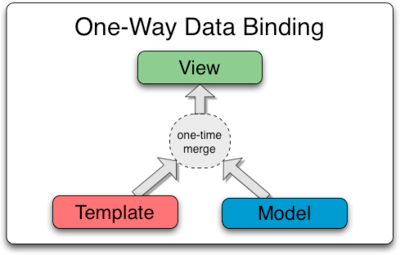
\includegraphics[width=\textwidth]{images/angularjs-one-way-data-binding.png}
\end{tcolorbox}

\subsubsection{Interpolation (from component to view)}

Interpolation binds a value from the TypeScript class to a section in the HTML.
\begin{verbatim}
<p>{{ title }}</p>
\end{verbatim}
In this example, the content of \texttt{title} in the component class is displayed inside the \texttt{<p>} element.

\subsubsection{Property Binding (from component to view)}

Property binding links an HTML element property to a component property.
\begin{verbatim}
<img [src]="imageUrl" alt="Dynamic image">
\end{verbatim}
Here, the \texttt{src} attribute of the image is bound to the \texttt{imageUrl} property in the component.

\subsubsection{Event Binding (from view to component)}

Event binding associates a DOM event (like a click) with a method in the component class.
\begin{verbatim}
<button (click)="onClick()">Click here</button>
\end{verbatim}
The \texttt{click} event triggers the \texttt{onClick()} method in the component when the button is clicked.

\subsection{Two-way Binding}

Two-way binding synchronizes data between the model and the view, so any change in one is immediately reflected in the other.
\begin{tcolorbox}[colframe=black!70, colback=white, title=Figure 6: Two-way Data Binding, fonttitle=\bfseries]
\centering
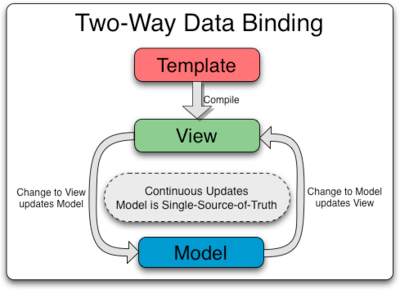
\includegraphics[width=\textwidth]{images/angularjs-two-way-data-binding.png}
\end{tcolorbox}

Angular primarily implements this using the \texttt{ngModel} directive, which binds a form field to a property in the component class.

\begin{verbatim}
<input [(ngModel)]="username">
<p>Username: {{ username }}</p>
\end{verbatim}

In this example, the value of \texttt{username} is bound to the input field. If the user types something, \texttt{username} is automatically updated, and if the \texttt{username} property changes in the component, the input field also updates.
\section{Using Angular Directives}

\textbf{Directives} are classes that modify the behavior of DOM elements. They are used to create reusable behaviors in the user interface.

\subsection{Structural Directives}

Structural directives modify the structure of the DOM by adding or removing elements. They are typically used to \textbf{control visibility} or \textbf{repeat elements}.

\subsubsection{*ngIf}

This directive conditionally displays a DOM element based on an expression. If the expression is true, the element is displayed; otherwise, it is removed from the DOM.
\begin{verbatim}
<div *ngIf="isVisible">This content is visible if isVisible is true.</div>
\end{verbatim}

\subsubsection{*ngFor}

This directive repeats an element for each item in a collection.
\begin{verbatim}
<ul>
  <li *ngFor="let item of items">{{ item }}</li>
</ul>
\end{verbatim}

\subsection{Attribute Directives}

Attribute directives modify the appearance or behavior of an element without changing its structure.

\subsubsection{ngClass}

This directive adds or removes CSS classes from an element based on conditions specified in the expression.
\begin{verbatim}
<div [ngClass]="{'highlight': isHighlighted}">This text is highlighted if isHighlighted is true.</div>
\end{verbatim}

\subsubsection{ngStyle}

This directive dynamically adds or modifies the styles of an element.
\begin{verbatim}
<div [ngStyle]="{'color': color, 'font-size': fontSize + 'px'}">This text has dynamic styles.</div>
\end{verbatim}

\section{Services and Dependency Injection}

\textbf{Services} play a critical role in Angular for managing \textbf{business logic}, accessing data, and performing external operations. They are used to provide reusable functionality throughout the application. Services are commonly used to communicate with APIs, manipulate data, or store information.
\begin{tcolorbox}[colframe=black!70, colback=white, title=Figure 7: Services and Dependency Injection, fonttitle=\bfseries]
\centering
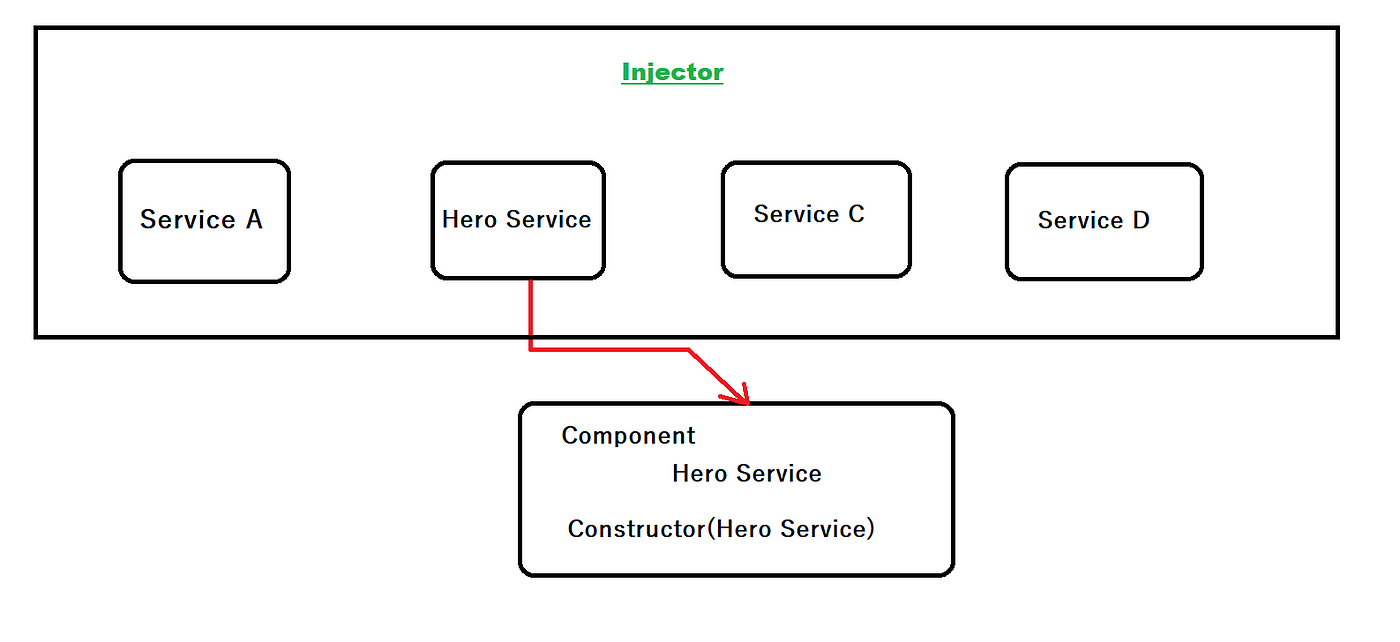
\includegraphics[width=\textwidth]{images/0_R0nqYsF51ACGiI_K.png}
\end{tcolorbox}

\subsection{Role of Services in Angular}

A service is a \textbf{class} that encapsulates specific logic or behavior. Services are often used to:
\begin{itemize}
  \item \textbf{Share data between components}: A service can store shared data and allow components to read or modify it.
  \item \textbf{Communicate with APIs}: A service can manage HTTP calls and retrieve data from a server.
  \item \textbf{Manage application state}: A service can hold information that needs to be accessible to multiple components, such as user authentication state or application settings.
\end{itemize}

\subsection{Dependency Injection with \texttt{@Injectable}}

\textbf{Dependency injection} (DI) is a core concept in Angular that allows injecting objects (such as services) into components or other services. This facilitates managing dependencies without requiring classes to create these objects themselves.

\subsubsection{\texttt{@Injectable()}}

This is a decorator that marks a class as an \textbf{injectable service}. It indicates to Angular that this class can be \textbf{injected} into other components or services.

Here is a simple example of a service with dependency injection:

\begin{lstlisting}[language=TypeScript, caption={TypeScript service example}, label={lst:typescript-service}]
import { Injectable } from '@angular/core';

@Injectable({
  providedIn: 'root' // This indicates that the service is available at the application level
})
export class DataService {
  private data: string[] = [];

  constructor() { }

  getData(): string[] {
    return this.data;
  }

  addData(newData: string): void {
    this.data.push(newData);
  }
}
\end{lstlisting}

\subsection{Using the Service in a Component}

In the component, you \textbf{inject} the service to access it:

\begin{lstlisting}[language=TypeScript, caption={Using a service in a component}, label={lst:typescript-service-usage}]
import { Component } from '@angular/core';
import { DataService } from './data.service';  // Import the service

@Component({
  selector: 'app-data-list',
  templateUrl: './data-list.component.html',
  styleUrls: ['./data-list.component.css']
})
export class DataListComponent {
  data: string[] = [];

  constructor(private dataService: DataService) { } // Inject the service

  ngOnInit(): void {
    this.data = this.dataService.getData();
  }

  addData(newData: string): void {
    this.dataService.addData(newData);
  }
}
\end{lstlisting}

In this example, \texttt{DataService} is injected into \texttt{DataListComponent} via the constructor. You can call the service's methods to retrieve or manipulate data. 

\section{Conclusion}

\begin{itemize}
  \item \textbf{Templates and Data Binding}: Data binding synchronizes the model (data) with the view (user interface). One-way and two-way bindings facilitate interaction between the model and the view.
  \item \textbf{Angular Directives}: Angular offers powerful directives like \texttt{*ngIf}, \texttt{*ngFor}, \texttt{ngClass}, and \texttt{ngStyle}, enabling declarative modifications to the DOM structure or styles.
  \item \textbf{Services and Dependency Injection}: Services encapsulate business logic and shared data. Dependency injection makes it easy to inject services into components, promoting modular and reusable code.
\end{itemize}

These fundamental Angular concepts are essential for developing robust and well-structured applications.
\section*{Routing in Angular}

\textbf{Routing} allows navigation between different views in an application. In Angular, routing is configured using the \texttt{RouterModule} and enables linking components to specific URLs.

\subsection*{1. Configuring Routes in \texttt{app-routing.module.ts}}

In Angular, routes are defined in a module file called \texttt{app-routing.module.ts}. This module imports the \texttt{RouterModule} and uses the \texttt{RouterModule.forRoot(routes)} method to configure the various routes.

Here is an example of route configuration:
\begin{lstlisting}[language=TypeScript, caption={Route Configuration Example}, label={lst:typescript-route-config}]
import { NgModule } from '@angular/core';
import { RouterModule, Routes } from '@angular/router';
import { HomeComponent } from './home/home.component';
import { AboutComponent } from './about/about.component';

const routes: Routes = [
  { path: '', component: HomeComponent },
  { path: 'about', component: AboutComponent }
];

@NgModule({
  imports: [RouterModule.forRoot(routes)],
  exports: [RouterModule]
})
export class AppRoutingModule { }
\end{lstlisting}

In this example:
- The default route (\texttt{path: ''}) loads the \texttt{HomeComponent}.
- The route \texttt{/about} loads the \texttt{AboutComponent}.

\subsection*{2. Navigating Between Components and Managing Route Parameters}

To navigate between components, the \texttt{routerLink} directive is used in the template, allowing URLs to be linked to an element.

Example:
\begin{verbatim}
<a routerLink="/about">About</a>
\end{verbatim}

\textbf{Managing Route Parameters}:
Sometimes, parameters need to be retrieved from the URL. This can be done using \texttt{ActivatedRoute} in the target component.

Example:
\begin{lstlisting}[language=TypeScript, caption={Retrieving Route Parameters}, label={lst:typescript-route-params}]
import { ActivatedRoute } from '@angular/router';

@Component({
  selector: 'app-about',
  templateUrl: './about.component.html',
  styleUrls: ['./about.component.css']
})
export class AboutComponent implements OnInit {

  constructor(private route: ActivatedRoute) { }

  ngOnInit(): void {
    this.route.params.subscribe(params => {
      const id = params['id']; // Retrieve the 'id' parameter from the URL
      console.log(id);
    });
  }
}
\end{lstlisting}

\section*{Forms in Angular}

Forms enable the collection of user input. Angular provides two main approaches for handling forms: \textbf{Template-Driven Forms} and \textbf{Reactive Forms}.

\subsection*{1. Template-Driven Forms}

In this approach, the form and its validations are primarily defined in the HTML template.

Example:
\begin{lstlisting}[language=HTML, caption={Template-Driven Form Example}, label={lst:template-driven-form}]
<form #myForm="ngForm" (ngSubmit)="onSubmit(myForm)">
  <input name="username" ngModel required />
  <button type="submit" [disabled]="!myForm.valid">Submit</button>
</form>
\end{lstlisting}

In this case, \texttt{ngForm} is a directive that creates a form object, and \texttt{ngModel} binds the fields to the component class.

\subsection*{2. Reactive Forms}

Reactive forms are more powerful and flexible. They are defined in the component and used to create complex forms with advanced validations.

Example:
\begin{lstlisting}[language=TypeScript, caption={Reactive Form Example}, label={lst:reactive-form}]
import { Component, OnInit } from '@angular/core';
import { FormBuilder, FormGroup, Validators } from '@angular/forms';

@Component({
  selector: 'app-login',
  templateUrl: './login.component.html',
  styleUrls: ['./login.component.css']
})
export class LoginComponent implements OnInit {

  loginForm: FormGroup;

  constructor(private fb: FormBuilder) { }

  ngOnInit(): void {
    this.loginForm = this.fb.group({
      username: ['', Validators.required],
      password: ['', [Validators.required, Validators.minLength(6)]]
    });
  }

  onSubmit(): void {
    if (this.loginForm.valid) {
      console.log(this.loginForm.value);
    }
  }
}
\end{lstlisting}

Here, \texttt{FormBuilder} is used to create a reactive form and apply validations to it.

\section*{Pipes in Angular}

\textbf{Pipes} are used to transform the data displayed in the user interface. They are commonly used to format values, such as dates or currencies.

\subsection*{1. Built-in Pipes}

Angular provides several built-in pipes for common transformations:
- \texttt{date}: Formats a date.
\begin{verbatim}
<p>{{ currentDate | date:'shortDate' }}</p>
\end{verbatim}

- \texttt{currency}: Displays a value as currency.
\begin{verbatim}
<p>{{ amount | currency:'EUR' }}</p>
\end{verbatim}

\subsection*{2. Creating Custom Pipes}

It is possible to create custom pipes for specific transformations required by the application.

Example:
\begin{lstlisting}[language=TypeScript, caption={Custom Pipe Example}, label={lst:custom-pipe}]
import { Pipe, PipeTransform } from '@angular/core';

@Pipe({
  name: 'reverse'
})
export class ReversePipe implements PipeTransform {
  transform(value: string): string {
    return value.split('').reverse().join('');
  }
}
\end{lstlisting}

In the template:
\begin{verbatim}
<p>{{ 'Hello' | reverse }}</p> <!-- Outputs 'olleH' -->
\end{verbatim}
\section*{Data Management and HTTP}

Angular enables HTTP requests using the \texttt{HttpClientModule}, making it easier to consume external APIs.

\subsection*{1. Using \texttt{HttpClientModule}}

To consume REST APIs, you first need to import the \texttt{HttpClientModule} in the \texttt{app.module.ts} file:

\begin{lstlisting}[language=TypeScript, caption={Importing HttpClientModule}, label={lst:typescript-httpclient-import}]
import { HttpClientModule } from '@angular/common/http';

@NgModule({
  imports: [HttpClientModule],
  // other configurations...
})
export class AppModule { }
\end{lstlisting}

Then, in your service or component, you can use \texttt{HttpClient} to make HTTP requests.

Example of a GET request:
\begin{lstlisting}[language=TypeScript, caption={HTTP GET Request Example}, label={lst:typescript-httpclient-get}]
import { HttpClient } from '@angular/common/http';

@Component({
  selector: 'app-data',
  templateUrl: './data.component.html',
  styleUrls: ['./data.component.css']
})
export class DataComponent {

  constructor(private http: HttpClient) {}

  fetchData(): void {
    this.http.get('https://api.example.com/data').subscribe(data => {
      console.log(data);
    });
  }
}
\end{lstlisting}

\subsection*{2. Consuming REST APIs and Error Handling}

When consuming APIs, it is important to handle errors using \texttt{catchError} and to process asynchronous responses.

Example of error handling:
\begin{lstlisting}[language=TypeScript, caption={Error Handling in HTTP Requests}, label={lst:typescript-httpclient-error}]
import { catchError } from 'rxjs/operators';
import { throwError } from 'rxjs';

this.http.get('https://api.example.com/data')
  .pipe(catchError(error => {
    console.error('Error occurred:', error);
    return throwError(error);
  }))
  .subscribe(data => {
    console.log(data);
  });
\end{lstlisting}

\section*{RxJS and Observables}

\textbf{Observables} are a core part of Angular and are used to handle asynchronous data streams, such as HTTP requests, user events, or data changes.

\subsection*{1. Introduction to RxJS}

RxJS (Reactive Extensions for JavaScript) is a library for composing asynchronous and event-based programs using observables.

An \textbf{observable} is a data stream that can be observed. A \textbf{subscriber} can subscribe to this observable to receive the emitted values.

Basic example with an observable:
\begin{lstlisting}[language=TypeScript, caption={Basic Observable Example}, label={lst:rxjs-basic-observable}]
import { Observable } from 'rxjs';

const observable = new Observable(subscriber => {
  subscriber.next('Hello');
  subscriber.complete();
});

observable.subscribe(value => console.log(value));  // Outputs 'Hello'
\end{lstlisting}

\subsection*{2. Using Observables to Handle Data Streams}

Observables allow you to manage data streams reactively, for example, handling data from an API, user events, etc.

Example with an HTTP request:
\begin{lstlisting}[language=TypeScript, caption={Using Observables for HTTP Requests}, label={lst:rxjs-http-observable}]
this.http.get('https://api.example.com/data')
  .subscribe(data => {
    this.data = data;
  });
\end{lstlisting}

\section*{Lazy Loading and Optimization}

\textbf{Lazy Loading} allows Angular modules to be loaded on demand, reducing the initial load time of the application.

\subsection*{1. Deferred Module Loading}

Lazy loading is configured in the routes. Instead of loading all modules at the start, only the necessary ones for the current view are loaded.

Example:
\begin{lstlisting}[language=TypeScript, caption={Lazy Loading Example}, label={lst:lazy-loading}]
const routes: Routes = [
  { path: 'dashboard', loadChildren: () => import('./dashboard/dashboard.module').then(m => m.DashboardModule) }
];
\end{lstlisting}

\subsection*{2. Performance Optimization}

Several techniques can improve the performance of an Angular application, such as:
- \textbf{Reducing bundle size} by using Lazy Loading.
- \textbf{Using ChangeDetectionStrategy.OnPush} to minimize change detection cycles.
- \textbf{Minification and compression of files} during deployment.
\section*{Testing and Deployment}

Unit testing ensures that the code works as expected, while deployment involves making the application available to users on a server or cloud platform.

\subsection*{1. Unit Testing with Jasmine/Karma}

Angular uses \textbf{Jasmine} for unit testing and \textbf{Karma} for running tests in a browser environment.

Example of a unit test:
\begin{lstlisting}[language=TypeScript, caption={Unit Test Example}, label={lst:typescript-unit-test}]
import { TestBed } from '@angular/core/testing';
import { DataService } from './data.service';

describe('DataService', () => {
  let service: DataService;

  beforeEach(() => {
    TestBed.configureTestingModule({});
    service = TestBed.inject(DataService);
  });

  it('should be created', () => {
    expect(service).toBeTruthy();
  });
});
\end{lstlisting}

\subsection*{2. Deploying to a Server or Cloud Platform}

Once the application has been developed and tested, it needs to be deployed to a server. The deployment process typically involves:
- Building the production version of the application with \texttt{ng build --prod}.
- Deploying the generated files (located in the \texttt{dist/} folder) to a server or a cloud platform such as \textbf{Firebase}, \textbf{AWS}, or \textbf{Heroku}.

\section*{Conclusion}

This course covers the essential concepts of Angular for creating robust and responsive applications. From routing to data management, forms, and performance optimization, Angular provides a comprehensive toolkit for modern web application development.

\end{document}
